\documentclass{article}

\usepackage[utf8]{inputenc}

\usepackage[citestyle=ieee,backend=biber,sorting=ynt]{biblatex}
\addbibresource{bibliography.bib}

\usepackage{hyperref}
\hypersetup{colorlinks=true,allcolors=blue}

\usepackage{appendix}
\usepackage{changepage}
\usepackage{enumitem}
\usepackage{graphicx}
\usepackage{tabularx}
\usepackage{xcolor,colortbl}

% \newcommand{\txvm}{\textsc{t}x\textsc{vm}}
\newcommand{\txvm}{TxVM}

\definecolor{smallint}{rgb}{1.0,1.0,0.9}
\definecolor{int}{rgb}{1.0,1.0,0.8}
\definecolor{stack}{rgb}{1.0,0.8,0.8}
\definecolor{value}{rgb}{1.0,0.8,1.0}
\definecolor{crypto}{rgb}{0.8,1.0,0.8}
\definecolor{tx}{rgb}{0.8,0.8,1.0}
\definecolor{flow}{RGB}{186,225,255}
\definecolor{ext}{rgb}{0.8,0.8,0.8}
\definecolor{data}{rgb}{1.0,0.9,0.8}
\definecolor{push}{RGB}{255,240,225}

\newenvironment{example}{
  \medskip\begin{adjustwidth}{.25in}{}\footnotesize
}{
  \normalsize\end{adjustwidth}
}

\newenvironment{commentary}{\begin{quote}\itshape}{\normalfont\end{quote}}

\title{\txvm{} \\ \large A New Design for Blockchain Transactions}
\date{March 2018}
\begin{document}
\author{
    \normalsize Bob Glickstein, Cathie Yun, Dan Robinson, Keith Rarick, Oleg Andreev \\
    \texttt{\normalsize \{bobg, cathie, dan, kr, oleg\}@chain.com} \\ \\
    Chain
}
\maketitle

\begin{abstract}

We present a new design for blockchain transactions called \txvm{},
the transaction virtual machine. \txvm{} seeks to achieve the
expressiveness and flexibility of an imperative contract model such as
Ethereum's while maintaining the efficiency, safety, and scalability of
a declarative transaction model such as Bitcoin's. \txvm{} defines a
stack machine for manipulating plain data items like strings,
integers, and tuples, but also special types: \textit{values}, each
with an amount and asset type; and \textit{contracts}, programs that
lock up values and other data. Rules governing the handling of these
types provide guarantees about integrity and security. Each
transaction is a \txvm{} program evaluated in isolation from the
blockchain state, and whose output is a deterministic log of proposed
state changes for the blockchain. Transactions can be therefore be
validated in parallel. Their logs can be applied to the blockchain in
linear time. Our implementation of \txvm{} is currently used in
production in our hosted ledger service, Sequence. The implementation
and specification are available as an open-source project on GitHub.

\end{abstract}

\section{Introduction}

A transaction in a blockchain protocol is a proposal to update the
blockchain's global state.  Depending on the blockchain, this could
mean consuming some value tokens and creating others, or updating the
balances in one or more accounts.  Participating nodes in the
blockchain network reach consensus on whether the transaction is valid
and should be applied. If so, the proposed state changes are made.

Different blockchain protocols take different approaches to
representing transactions, each with its own strengths and weaknesses.

\subsection{Prior art: Bitcoin}

In Bitcoin \cite{nakamoto} and similar systems, including earlier
versions of the Chain Protocol, a transaction is a static data
structure with fields that must be interpreted and validated using an
ad hoc collection of rules. One or more ``inputs'' identify existing
tokens to be redeemed from earlier transactions. Each input includes
the data needed to authorize access to those tokens. The accessed
value is divided among one or more ``outputs.'' Each describes how to
secure its value. This is typically done by specifying the public key
of a payee, usually in the form of a short program for a specialized
virtual machine. The program verifies a digital signature against that
public key. Some future ``input'' must supply that signature to
``spend'' the output.

This model is \textbf{declarative}. The transaction's data structure
declares its proposed state changes directly. No user-defined program
runs except for the predicates attached to the previous outputs to
authorize their use, and there are no effects on the blockchain state
other than the ones discoverable by a simple inspection of the
transaction's fields. Furthermore, tokens are immutable. Once created,
they persist in the same state until consumed.

These properties make declarative transactions efficient and
secure. Transactions can be validated in parallel before any of their
effects have to be applied to the blockchain state.\footnote{One transaction's application to the state may render another
transaction inapplicable, as when each tries to spend the same
token. For our purposes, this is a separate step from validation, and is considered acceptable as long as such conflicts can be resolved in approximately linear time.} It
is easy to avoid transactions with unexpected side-effects. And the global blockchain state does not need to contain much more than a cryptographic hash committing to the contents of each existing token.

On the other hand, Bitcoin's transaction model limits the power of its
smart contracts. This is partially a result of Bitcoin's restricted
virtual machine, which by design is not Turing-equivalent. But mainly
it's because Bitcoin's scripts are simple predicates evaluated
independently of each other. This makes it unduly difficult to express
multiple contracts interacting, even after adding more powerful
opcodes, as in earlier versions of the Chain Protocol. We found that
modeling more sophisticated flows of value required unwieldy
contortions in the best case and were occasionally impossible to do
securely.

\subsection{Prior art: Ethereum}

In Ethereum \cite{wood2014ethereum} and similar systems, value resides
in contracts that also embody mutable state and program logic. A
transaction is a message sent to a contract, causing its program to
execute.

This is an \textbf{imperative} model, in which the effects of the transaction on the blockchain are not known until the contract logic finishes running, during which time it may alter its own state as well as send messages to other contracts, which can update their own state.

Contract logic may be highly sophisticated, and indeed a wide variety of novel flows of value have been demonstrated using imperative blockchain contracts, from decentralized autonomous organizations to cryptocurrency-based virtual pets.

However, interaction with the global blockchain state during execution
means that there can be no meaningful optimization by parallelizing
validation. Transactions must execute serially, in a deterministic
order. Since one contract might alter the state of any other contract,
it is easy for execution to have unexpected side-effects, and it can
be difficult to reason about a contract's state even during the
lifetime of a single transaction. This can be catastrophic, such as in
the June~2016 hack of the ``DAO'' contract \cite{dao}, which resulted
in the theft of around \$50~million, and the November~2017 Parity bug
\cite{parity}, which froze wallets containing around \$150~million.

\subsection{A combined approach}

\txvm{} is the basis for the protocol used in Sequence
\cite{sequence}, Chain's blockchain-based hosted ledger
service. \txvm{} stands for ``transaction virtual machine.''

With \txvm{} we seek to combine the respective strengths of the
declarative and imperative approaches to representing blockchain
transactions, while avoiding their weaknesses. It takes advantage of
lessons we learned from our own previous design, ChainVM
\cite{chainvm}, and from developing Ivy \cite{ivy}, our higher-level
smart-contract language, which compiles to ChainVM and also to Bitcoin
Script. \txvm{} is designed to be an ideal compilation target for Ivy.

A \txvm{} transaction is an \textbf{imperative} program that produces
a \textbf{declarative} log of proposed blockchain state changes when
executed. Execution happens in isolation from the global blockchain
state. Running in isolation means \txvm{} programs cannot have
unexpected side effects in other contracts, and that they can be run
in parallel.

\section{Operation of the virtual machine}

\txvm{} defines a stack-based virtual machine to execute transaction
programs. Programs are expressed as strings of bytecode. The \txvm{}
instruction set includes a \texttt{jumpif} instruction, making it
Turing-complete. It also includes operations for manipulating various
types of data, introspecting aspects of the VM state, computing
cryptographic hashes, verifying signatures, and more. The complete
instruction set is shown in figure~\ref{instset}.

\newcolumntype{C}{>{\centering\arraybackslash}X}
\begin{figure}
\def\arraystretch{1.5}
\setlength\tabcolsep{5pt}
\centering\ttfamily\scriptsize
\begin{tabularx}{\textwidth}{lCCCCCCCC}
& 00 & 10 & 20 & 30 & 40 & 50 & 60 & 70 \\
0 & \cellcolor{smallint} 0/false & \cellcolor{smallint} 16 & \cellcolor{int} int       & \cellcolor{value} nonce     & \cellcolor{flow} verify        & \cellcolor{data} eq      & \cellcolor{push} 1 byte   & \cellcolor{push} 17 bytes \\
1 & \cellcolor{smallint} 1/true  & \cellcolor{smallint} 17 & \cellcolor{int} add       & \cellcolor{value} merge     & \cellcolor{flow} jumpif        & \cellcolor{data} dup     & \cellcolor{push} 2 bytes  & \cellcolor{push} 18 bytes \\
2 & \cellcolor{smallint} 2         & \cellcolor{smallint} 18 & \cellcolor{int} neg       & \cellcolor{value} split     & \cellcolor{flow} exec          & \cellcolor{data} drop    & \cellcolor{push} 3 bytes  & \cellcolor{push} 19 bytes \\
3 & \cellcolor{smallint} 3         & \cellcolor{smallint} 19 & \cellcolor{int} mul       & \cellcolor{value} issue     & \cellcolor{flow} call          & \cellcolor{data} peek    & \cellcolor{push} 4 bytes  & \cellcolor{push} 20 bytes \\
4 & \cellcolor{smallint} 4         & \cellcolor{smallint} 20 & \cellcolor{int} div       & \cellcolor{value} retire    & \cellcolor{flow} yield         & \cellcolor{data} tuple   & \cellcolor{push} 5 bytes  & \cellcolor{push} 21 bytes \\
5 & \cellcolor{smallint} 5         & \cellcolor{smallint} 21 & \cellcolor{int} mod       & \cellcolor{value} amount    & \cellcolor{flow} wrap          & \cellcolor{data} untuple & \cellcolor{push} 6 bytes  & \cellcolor{push} 22 bytes \\
6 & \cellcolor{smallint} 6         & \cellcolor{smallint} 22 & \cellcolor{int} gt        & \cellcolor{value} assetid   & \cellcolor{flow} input         & \cellcolor{data} len     & \cellcolor{push} 7 bytes  & \cellcolor{push} 23 bytes \\
7 & \cellcolor{smallint} 7         & \cellcolor{smallint} 23 & \cellcolor{int} not       & \cellcolor{value} anchor    & \cellcolor{flow} output        & \cellcolor{data} field   & \cellcolor{push} 8 bytes  & \cellcolor{push} 24 bytes \\
8 & \cellcolor{smallint} 8         & \cellcolor{smallint} 24 & \cellcolor{int} and       & \cellcolor{crypto} vmhash   & \cellcolor{flow} contract      & \cellcolor{data} encode  & \cellcolor{push} 9 bytes  & \cellcolor{push} 25 bytes \\
9 & \cellcolor{smallint} 9         & \cellcolor{smallint} 25 & \cellcolor{int} or        & \cellcolor{crypto} sha256   & \cellcolor{flow} seed          & \cellcolor{data} cat     & \cellcolor{push} 10 bytes & \cellcolor{push} 26 bytes \\
a & \cellcolor{smallint} 10        & \cellcolor{smallint} 26 & \cellcolor{stack} roll    & \cellcolor{crypto} sha3     & \cellcolor{flow} self          & \cellcolor{data} slice   & \cellcolor{push} 11 bytes & \cellcolor{push} 27 bytes \\
b & \cellcolor{smallint} 11        & \cellcolor{smallint} 27 & \cellcolor{stack} bury    & \cellcolor{crypto} checksig & \cellcolor{flow} caller        & \cellcolor{data} bitnot  & \cellcolor{push} 12 bytes & \cellcolor{push} 28 bytes \\
c & \cellcolor{smallint} 12        & \cellcolor{smallint} 28 & \cellcolor{stack} reverse & \cellcolor{tx} log          & \cellcolor{flow} cprog. & \cellcolor{data} bitand  & \cellcolor{push} 13 bytes & \cellcolor{push} 29 bytes \\
d & \cellcolor{smallint} 13        & \cellcolor{smallint} 29 & \cellcolor{stack} get     & \cellcolor{tx} peeklog      & \cellcolor{flow} timerange     & \cellcolor{data} bitor   & \cellcolor{push} 14 bytes & \cellcolor{push} 30 bytes \\
e & \cellcolor{smallint} 14        & \cellcolor{smallint} 30 & \cellcolor{stack} put     & \cellcolor{tx} txid         & \cellcolor{ext} prv            & \cellcolor{data} bitxor  & \cellcolor{push} 15 bytes & \cellcolor{push} 31 bytes \\
f & \cellcolor{smallint} 15        & \cellcolor{smallint} 31 & \cellcolor{stack} depth   & \cellcolor{tx} finalize     & \cellcolor{ext} ext            & \cellcolor{push} 0 bytes & \cellcolor{push} 16 bytes & \cellcolor{push} 32 bytes \\
\end{tabularx}

\normalfont\medskip

\def\arraystretch{1.7}
\begin{tabular}{ccccc}
\cellcolor{smallint} small ints & \cellcolor{stack} stack ops & \cellcolor{crypto} crypto ops & \cellcolor{flow} control flow & \cellcolor{data} data ops \\
\cellcolor{int} int ops         & \cellcolor{value} value ops & \cellcolor{tx} tx ops         & \cellcolor{ext} extension     & \cellcolor{push} pushdata \\
\end{tabular}

\normalsize

% 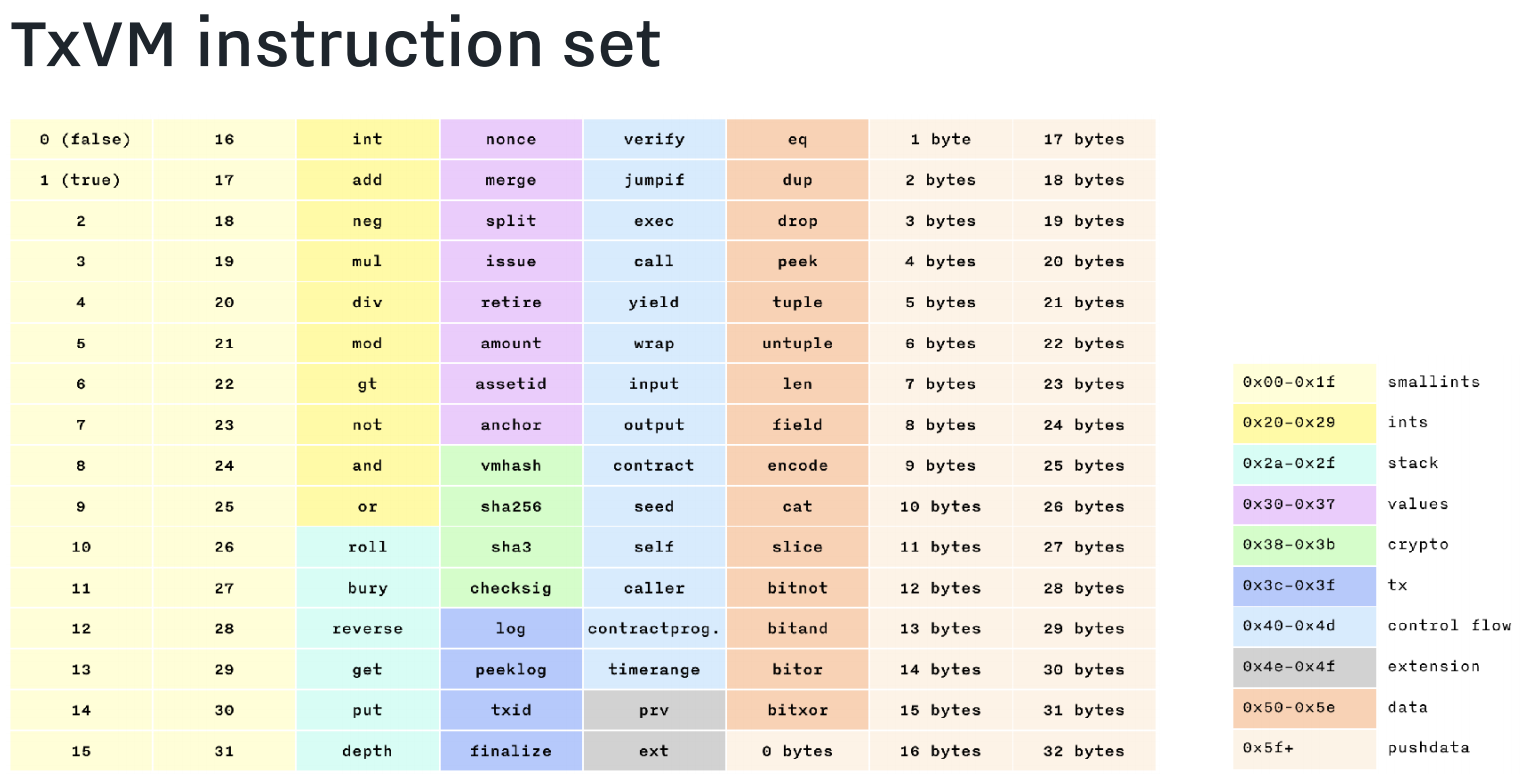
\includegraphics[width=\textwidth]{instset.png}
\caption{The TxVM instruction set.}
\label{instset}
\end{figure}

Certain instructions cause records to be appended to the
\textit{transaction log}, a VM data structure that is the primary
output of running a \txvm{} program. It contains the blockchain state
changes proposed by the transaction. After the transaction program
finishes, the log may be applied to the blockchain.

A \textit{contract} is a unit of program execution that contains a
program (a string of bytecode) and a stack. While a contract is
running, its stack serves as the VM's \textit{current contract stack},
where most stack-based operations take place. A contract may also
suspend its execution in a variety of ways, passing control to some
other contract. At such times the suspended contract's stack is
preserved until it is reinvoked.

When control passes from one contract to another, data may be passed
between them on the VM's shared \textit{argument stack}.

The overall transaction program forms an implicit top-level contract.

Stacks may contain plain data items: strings, integers, and
tuples. They may also contain contracts, and they may contain
\textit{values}, each of which is a specific amount of a specific
asset type. Values and asset types are discussed in further detail in
the next section.

In addition to their bytecode, transaction programs specify an integer
\textit{runlimit}. Each instruction costs a nonzero amount to execute,
and the total cost of running the program must not exceed the
specified runlimit. This prevents abuse of the network in a similar
way to the role played by Ethereum's ``gas.'' A network can agree to
reject transactions with runlimits that are too high.

In order to be valid, a transaction program must execute to completion
and leave no data on any stack.

\subsection{Values}

A \txvm{} blockchain is used to track the issuance, ownership, and
transfer of values of different types and amounts, e.g. ``5 USD'' or
``3 shares of AAPL.'' A value is a first-class item on the stack.

Inside a value object is an amount, an \textit{asset~ID}, and an
\textit{anchor}. A new value may be created only by the \texttt{issue}
instruction, which populates the asset~ID field with a cryptographic
hash computed from the currently running contract---the one containing
the \texttt{issue} instruction. An issuance contract thus uniquely
determines the asset type it issues. No other contract may issue units
of the same asset.

The \texttt{issue} instruction populates the anchor field with a hash
derived from earlier values in the blockchain, guaranteeing uniqueness
and non-replayability.

Finally, \texttt{issue} adds a record of the new issuance to the
transaction log.

Once created, a value may be \texttt{split} into two values with the
same asset~ID and sum, and may be \texttt{merge}d with other values
with the same asset~ID, in all cases producing values with new
anchors. A value with an amount of zero is useful in some cases for
its anchor alone.

Values may be destroyed with the \texttt{retire} instruction, which
also creates a transaction log record.

Unlike plain data, values may not be duplicated or dropped from a
stack.

\subsection{Contracts}

A contract contains a program and a stack. It is created with the
\texttt{contract} instruction. Its stack is initially empty, and its
program is set to the bytecode string that \texttt{contract} takes as
an argument.

Contracts are invoked with \texttt{call}, which causes the VM's
current contract stack to be saved away and replaced by the called
contract's stack. The saved stack is restored when control returns to
the caller.

When a contract reaches the end of its program with an empty stack, it
is \textit{complete}. It is removed from the VM and control returns to
the caller. It is an error for a contract to reach the
end of its program while items remain on its stack. If it is the implicit top-level contract, the argument
stack must also be empty.

A contract that has not yet completed may suspend its own execution in
one of three ways:

\begin{itemize}

\item It may execute the \texttt{yield} instruction, placing the
  contract on the argument stack while returning control to the
  caller.

\item It may execute the \texttt{output} instruction, writing an
  ``output'' record to the transaction log. That record contains a cryptographic hash committing to a snapshot of the contract's state, including the contents of its stack. This \textit{snapshot hash} will be added to the
  blockchain's global state as an unspent output contract. The
  contract may be reconstituted in a later transaction, and its
  execution resumed, with the \texttt{input} instruction.

\item It may execute the \texttt{wrap} instruction, which is like
  \texttt{yield} but makes the suspended contract ``portable.''
  Portability of contracts is not discussed here; for details please
  see the \txvm{} spec. \cite{txvm-spec}

\end{itemize}

In order to reconstitute a contract from the global blockchain state
(placed there with \texttt{output}), a program first creates a
plain-data depiction of the contract: a tuple that includes the
contract's program string and all the items on its
stack.\footnote{Since only the snapshot hash is stored in the
blockchain state, the user has the responsibility to remember or
retrieve sufficient information about the contract to reconstruct
it. This may involve monitoring the blockchain for recognizable
contract patterns and parsing those, communicating out-of-band with
the contract's creator, or other techniques.}  The \texttt{input}
instruction turns that tuple into a callable contract object while
adding an ``input'' record to the transaction log. The input record
contains a snapshot hash computed from the tuple. Later, when the log
is applied to the blockchain, that snapshot hash is checked against
the global state to ensure that the stipulated contract actually
exists to be consumed.

Like values, contracts may not be duplicated or dropped from a
stack. Thus, all contracts created during a transaction must run to
completion or be persisted to the global blockchain state with
\texttt{output} in order to be cleared from the~VM. It follows too
that all values (other than those that are destroyed with
\texttt{retire}) must end up in the stack of a contract persisted with
\texttt{output}, or else be left in the VM, preventing successful
completion.

\subsection{The transaction log}

The transaction log is the primary result of running a \txvm{}
transaction. It is also the source of a transaction's unique~ID, which
is computed from a hash of the log's contents.

A transaction usually includes one or more signature checks. The
message being signed is typically the transaction's~ID, possibly in
combination with other data. This creates a chicken-and-egg problem:
the transaction is not complete until it includes the necessary
signatures, but the signatures require the transaction~ID, which
requires running the transaction.

To solve this problem, \txvm{} includes the \texttt{finalize}
instruction. This freezes the transaction log, prohibiting further
changes to it. It also makes the \texttt{txid} instruction available
for querying the transaction's~ID. Every transaction must execute
\texttt{finalize} exactly once. It is possible to run a transaction
program up to its \texttt{finalize} instruction, in order to compute
the~ID of that transaction. Signature-checking contracts presumably
still remain on the stack at this point.  Once the~ID has been
computed, it's possible to compute any required signatures.  These can
now be added to the transaction program as arguments to those
contracts, together with the \texttt{call} instructions that will
invoke them and clear them from the~VM.

To ensure the uniqueness of each transaction and each transaction~ID,
the \texttt{finalize} instruction consumes an anchor (a value with an
amount of zero) from the stack.

\section{A typical transaction}

In this section we present a simplified \txvm{} transaction, in which
Alice wishes to pay~10 units of some asset to Bob. Alice's transaction
inputs two contracts from the blockchain, one containing~5 units and
the other containing~7. The transaction combines those values and then
resplits them, creating one output of~10 for Bob and a ``change''
output of~2 for Alice.

This example uses \txvm{} assembly-language notation, in which certain
operations have a simplified depiction. For instance, ``pushdata''
instructions are implicit, tuple literals (delimited as
\texttt{\{...\}}) abbreviate the steps needed to construct them, and a
sequence of assembly-language instructions enclosed in square brackets
(\texttt{[...]}) denotes the bytecode string they produce when
assembled.

Here is the transaction, with some details elided for clarity.

\begin{example}

\begin{verbatim}
{...} input call get get
{...} input call get get
\end{verbatim}

\begin{commentary}
Marshal two contracts from the global blockchain state, call them, and
move their results---a value and a signature-check contract
each---from the argument stack to the current contract stack.
\end{commentary}

\begin{verbatim}
2 roll merge
\end{verbatim}

\begin{commentary}
Put the two values (a 5-unit value and a 7-unit value) next to each
other on the stack and merge them into one 12-unit value.
\end{commentary}


\begin{verbatim}
10 split <Bob's pubkey> put put [get get ... output] contract call
\end{verbatim}

\begin{commentary}
Split the 12-unit value into one 10-unit value and one 2-unit
value. Add Bob's pubkey to the stack. Move it and the 10-unit value to
the argument stack. Construct and call a contract whose program
consumes the value and pubkey, then {\normalfont\texttt{output}}s
itself.
\end{commentary}

\begin{verbatim}
2 split <Alice's pubkey> put put [get get ... output] contract call
\end{verbatim}

\begin{commentary}
Split the 2-unit value into one 2-unit value and one zero-unit value
(which will be used as an anchor by
{\normalfont\texttt{finalize}}). Add Alice's pubkey to the stack.
Construct and call a contract whose program consumes the value and
pubkey, then {\normalfont\texttt{output}}s itself.
\end{commentary}

\begin{verbatim}
finalize
\end{verbatim}

\begin{commentary}
Consume the zero-value anchor and freeze the transaction log. At this
point, the two signature-check contracts (for authorizing the
{\normalfont\texttt{input}}s above) remain on the stack.
\end{commentary}

\begin{verbatim}
<a signature by Alice of this transaction ID> put call
<a signature by Alice of this transaction ID> put call
\end{verbatim}

\begin{commentary}
Supply a signature to each signature-check contract and call it to
clear it from the~VM.
\end{commentary}

\end{example}

The next sections take a look at some of the details elided from the
example above.

\subsection{Checking signatures}

Here is a simple signature-checking program.

\begin{verbatim}
txid <pubkey> get 0 checksig verify
\end{verbatim}

The steps of this program are:

\medskip

\begin{tabular}{rp{0.75\textwidth}}
\texttt{txid}     & Get the transaction's ID and push it on the stack (only possible after \texttt{finalize}); \\
\textit{pubkey}   & Push the pubkey (of a value's owner, or an asset's authorized issuer, etc\@.) on the stack; \\
\texttt{get}      & Move a data item (the signature) from the argument stack to the current contract stack; \\
\texttt{0}        & Push a~0 on the stack (signaling the \texttt{checksig} instruction to use the Ed25519 signature scheme); \\
\texttt{checksig} & Compute the validity of the signature with respect to the transaction~ID and pubkey; \\
\texttt{verify}   & Fail execution if \texttt{checksig} did not produce a true value. \\
\end{tabular}

\subsection{Unspent output}

Here is a simple program for an unspent output contract that already
contains a value and a payee's pubkey on its stack.

\begin{verbatim}
put [txid swap get 0 checksig verify] yield
\end{verbatim}

The \texttt{put} instruction releases the contract's value to the
argument stack. The \texttt{yield} instruction, with a
signature-checking program as an argument, suspends this contract's
execution (with the payee's pubkey still on its stack) and places
\emph{it} on the argument stack. Of course, the suspended contract
will need to be \texttt{call}ed again to clear it from the~VM. This is
a \textit{deferred} signature check, which can run only after
\texttt{finalize}, since it uses \texttt{txid}.

Note that this version of the signature-checking contract differs
slightly from the example presented above. In that example, the pubkey
appears literally in the program. In this example, the pubkey is
already on the stack and is moved into its proper place (with
\texttt{swap}\footnote{Which is \txvm{} assembly-language shorthand
  for \texttt{1~roll}.}) after the transaction~ID is placed on the
stack.

Knowing this program, it is possible to flesh out some of the tuple
passed to \texttt{input}:

\begin{verbatim}
{'C',
  <seed>,
  [txid swap get 0 checksig verify],
  <payee pubkey>,
  {'V', <amount>, <asset ID>, <anchor>}
}
\end{verbatim}

Here, \texttt{C} and \texttt{V} are type codes (for ``contract'' and
``value'' respectively), and ``seed'' is the contract's seed, a unique
identifier (not discussed here). The \texttt{input} instruction turns
this structure into a contract object, meanwhile computing a snapshot
hash for the transaction log that must match the snapshot hash from an
earlier \texttt{output} instruction.

\subsection{Pay-to-pubkey}

Finally, here is the contract used to lock up value with a payee's
pubkey. Note how the unspent-output contract is a latter phase of this
contract, and the signature check is a latter phase of \emph{that}.

\begin{verbatim}
get get [put [txid swap get 0 checksig verify] yield] output
\end{verbatim}

This consumes two arguments from the argument stack, a pubkey and a
value. It then \texttt{output}s itself as an unspent-output
contract. When next called (after \texttt{input}), it will release the
value and defer a signature check against the pubkey.

\subsection{Scratching the surface}

The example in this section is a simplified transfer of a single type
of value from a single sender to a single recipient. In Sequence such
transfers are made with slightly more elaborate versions of the
contract programs presented here. Those programs include provisions
for M-of-N signatures and for attaching user-supplied reference data
to payments, among other things.

Beyond that, it should be evident that much more is possible. A
transaction can involve multiple parties trading multiple asset types
simultaneously and atomically. A contract can lock up zero, two, or
more values, not just one.  An asset's issuance contract can be
designed to constrain how units of it may be spent.

A discussion of TxVM's full power is beyond the scope of this paper;
indeed we are still discovering it ourselves. In the coming months we
will be retargeting our compiler for the Ivy high-level smart contract
language to TxVM. We expect to show how use cases such as escrowed
payments, collateralized loans, second-price auctions, bond coupons,
and even decentralized autonomous organizations and
cryptocurrency-based virtual pets may be expressed in Ivy and compiled
to compact TxVM programs.

\section{Further reading}

We have a full specification and implementation of \txvm{} available
as an open-source project on GitHub, at
\href{https://github.com/chain/txvm}{\texttt{github.com/chain/txvm}}.

One of us (Yun) presented \txvm{} at the Stanford Blockchain Protocol
Analysis and Security Engineering (\textsc{bpase}) 2018
conference. \cite{bpase} The talk and slides are available
online. \cite{txvm-talk} \cite{txvm-slides}

\txvm{} is currently being used in production in our ledger service,
Sequence. For more information, visit
\href{http://www.chain.com}{\texttt{Chain.com}} and read our blog
post, ``Introducing Sequence.'' \cite{sequence}

\section{Conclusion}

We have presented \txvm{}, a transaction model and virtual-machine design that combines the usability and power of Ethereum-like contracts with the safety, efficiency, and scalability of Bitcoin-like transactions.

We designed \txvm{} to serve as the core of our platform for financial applications. We have a full specification and open-source implementation of \txvm{} in Go, currently deployed in production.

Beyond continuing to use \txvm{} in production and developing it
further, we are interested in applying these ideas to other blockchain
protocols. Constructive transaction programs may provide novel ways to
build and serialize transactions in Bitcoin-like protocols, while
declarative deterministic effect logs may improve the safety and
scalability of Ethereum-like platforms.

\newpage

\printbibliography

\end{document}
